\chapter{Topic Extraction Engine} \label{ch:4:topic}

The semantic analysis tool shown in~\Cref{fig:sys_arch} focuses on 2 main text mining components in order to extract information from the news articles. This section focuses on the first of these components: the topic extraction engine, covering different data processing techniques, word and document approaches, semantic clustering and topic modelling using LDA. 

\section{Data Processing} \label{s:procesing_topic_engine}

The prepared data (from~\Cref{dataloader}) grouped by (Year, Category) comprises of a list of articles that were published in that year and belong to the category. Processing all the text for every single article would result in intensive computational burden without a huge amount of added benefit, as well as a potential risk of cluttering the model. For the sake of brevity, the aim was to use the article data most representative of the article. To facilitate this, a decision was made to use the titles and introduction of the articles as they contain the core information in the articles. The introduction of the article (`intro') was extracted as the first 8 sentences of the article using spaCy's \texttt{SentenceSplitter}. Throughout the course of this chapter, `intro' and `article' will be used inter-changeably to represent a single news article in the corpus. 

Once the article introductions (`intros') are extracted, they then undergo pre-processing before they can be vectorised for clustering. This section highlights the different pre-processing steps and key decisions made to convert the article intros into a list of tokens for the vectorisation step.

\subsection{Coreference Resolution} \label{coref}
The first step involves coreference resolution of the articles (`intros'). This involves using the pre-trained AllenNLP SpanBERT coreference resolution model for finding the set of mentions in the text that refer to the same `entity' (i.e. coreference clusters). This step was performed on the complete article intro in order for the mentions to be resolved throughout the entirety of the intro and not just on a sentence level. For example, for the sentences ``Sean Doyle is the CEO of British Airways. Prior to this, he was the CEO of Air Lingus'', if the coreference resolution was done at the sentence level, the model would miss out on resolving `he' in the second sentence to `Sean Doyle'.

\subsection{Cleaning Data} \label{data_cleaning}
Post-coreference resolution of the article intros, the data needs to be `cleaned' in order to ensure that the news articles retrieved are informative and useful. This involves the following steps: 
\begin{enumerate}
    \item Removing any unnecessary characters e.g., trailing ellipsis, parenthesis etc.
    \item Removing stopwords using spaCy's default stopword list for the pre-trained English model, containing words such as `its', `moreover', `that', `are' etc. This stoplist is augmented with a custom list of words such as \qs{told}, \qs{said}, \qs{airline}, \qs{flight} etc. which, given the nature of our dataset, online articles for airline industry, occur in the majority of the articles. These words do not contribute towards any relevant information specific to the article and are therefore removed in attempt to reduce redundancy. Similarly, common phrases in online articles such as \qd{Read here}, \qd{For more information} etc. are also removed. This significantly reduced the amount of text per article.

\end{enumerate}

\subsection{Named Entity Recognition}
As mentioned previously, the aim of these pre-processing steps was to obtain a \texttt{filtered\_tokens} list for each article intro which would be vectorised to represent an article as a vector for clustering. A key decision made was to remove all corresponding named entities from the `article intro' in order to remove any dependency of the topics on these named entities. Eliminating this dependency resulted in better silhouette scores and coherence scores for semantic clustering and topic extraction as detailed in~\Cref{s:preprocess_clustering} and~\Cref{s:preprocess_topic} respectively. 

This step was done before tokenisation as named entities are often multi-word entities such as ``British Airways", ``Paul Sweeney", ``New Haven" etc. and removing these post-tokenisation would not be ideal as they would lose their semantic meaning as tokens. For instance, post tokenisation, the model would try to remove all instances of `New' and `Haven' from the `article intro'. Therefore, regex patterns were used to remove all the occurrences of the extracted entities in an article. This included removing all entity types (See Appendix~\Cref{appendix:semantic_types}) which included, but were not limited to, `PER', `LOC', `GPE', `MONEY', `DATE', `ORG' etc. This also had a performance gain over the post-tokenisation approach as it avoided the lookup for each token against the unwanted entity tokens list.

The process of extracting the named entities from the article corpus involved using the Fine Grained NER model (See~\Cref{s:models}) and the BILOU encoding scheme for NER (See~\Cref{named_ents}) and is detailed in~\Cref{alg:named_ents}. The output from the NER model gives a set of words and their corresponding entity tags. In essence, the algorithm shows the process of obtaining single word entities (with `Unit' tag) and multi-word entities (by joining entity tokens to build the entity phrases starting from the `Beginning' token until the `Last' token) and ignoring words with the `Outside' tag as they do not refer to an entity.

\begin{algorithm}[H]
  \caption{Extract Named Entities}
  \label{alg:named_ents}
  \begin{algorithmic}   
  \State $\mathit{entities} \leftarrow \emptyset$
  \State $\mathit{words, tags} \leftarrow \mathit{ner\_model.predict}(sentence)$
  \ForAll{$\mathit{word, tag} \in \mathit{zip(words, tags)}$ } 
    \If{$t == $ `$O$'}  \State {$continue$}  \EndIf
    \State $ \mathit{ent\_position, ent\_type} = \mathit{tag.split}(\text{`--'})$
    \If{$t == $ `$U$'} 
    \State{$\mathit{entities.add(word)}$}
    \Else
      \If{ $\mathit{ent\_position} == $ `$B$'} 
      \State $ent := word$
      \ElsIf { $\mathit{ent\_position} == $ `$I$'} 
      \State  $\mathit{ent:= ent + word}$
      \ElsIf { $ent\_position == $ `$L$'} 
      \State  $\mathit{ent := ent + word} $
      \State{$\mathit{entities.add(ent)}$}
      \EndIf
    \EndIf
  \EndFor
\end{algorithmic}
\end{algorithm}

\subsection{Filtering Tokenised Data} \label{filtered_tokens}
Once the data is cleaned and void of the pre-determined entity types, the article intros are tokenised and normalised. This was done using the spaCy library's \texttt{Tokeniser} and \texttt{Lemmatiser} respectively, which are pre-trained on the English language model: \texttt{en\_core\_web\_lg} (See~\Cref{libraries}). Normalisation was done through lemmatisation (to obtain the base forms of the tokens). This was chosen instead of stemming as it guaranteed more semantically meaningful tokens for reasons detailed in~\Cref{normalisation}. The process of obtaining a list of tokens for each article intro was as follows:
\begin{enumerate}
    \item Each sentence in the intro was turned into a list of tokens.
    \item These tokens were filtered by their Part-Of-Speech (POS) tags against the allowed POS tags, which was restricted to nouns (`NOUN').
    \item Tokens that were numeric and less than 2 characters were also removed. 
    \item The remaining tokens were lemmatised and added to the \texttt{filtered\_tokens} list for the given article.
\end{enumerate}

It is important to note that the allowed POS tags were originally set to include nouns (NOUN), adjectives (ADJ), verbs (VERB) and adverbs (ADV). This resulted in a lot of unnecessary tokens such as `because', `did', `very' etc. Different combinations of the allowed POS tags were experimented with, ultimately allowing only nouns to comprise the \texttt{filtered\_tokens} for each article (`intro'). This decision was primarily based on the resulting clustering scores when the allowed POS tags were limited to `NOUN' and when they included `NOUN', `ADJ', `VERB' and `ADV' as discussed in the evaluation in~\Cref{s:pos_clustering}.

\section{Semantic Clustering} \label{s:semantic_clustering}

The first step to generating semantic clusters of articles is to get the corresponding article vectors. This involves vectorising the individual tokens in \texttt{filtered\_tokens} list for each article intro.

\subsection{Word embedding approaches} \label{word_embed_approaches}
To vectorise the tokens, different pre-trained word embedding models were used. These approaches (in chronological order) with their strengths and shortcomings are outlined below.

\renewcommand\arraystretch{2}
\captionsetup{singlelinecheck=false, labelfont=sc, labelsep=quad}
\begin{longtable}{@{\,}r <{\hskip 2pt} !{\foo} >{\arraybackslash}p{14cm}}
\centering

TF-IDF & Term Frequency-Inverse Document Frequency is a statistical metric that examines the comparative relevance of a word/token with respect to an article intro in the collection of articles. Representing the tokens as their TF-IDF measure first involves calculating the term frequency (TF) using the bag of words (BoW) approach from Gensim \texttt{Doc2BoW}. To account for overlapping terms across all article intros, the term frequency was multiplied by the inverse document frequency to weigh down the terms whose high frequency is not unique to a document (Refer to~\Cref{types_embeddings}). A dense document-term using the TF-IDF values for each term is used to represent the article intro as a vector for clustering. \\

Word2Vec & The next approach saw the use of Google's \texttt{Word2Vec} model (from Gensim) to obtain pre-trained word embeddings for each token in an article's corresponding \texttt{filtered\_tokens} list. The issue with the previous approach was that it represented the statistical information about a document, in particular, the measure of the frequency of words in a document, rather than any semantic information about a document. \texttt{Word2Vec} embeddings, on the other hand, return a vector for each word that accounts for semantic similarity (based on cosine distance) between the words represented by the vectors~\cite{word2vec}. \\

GloVe & The final approach was to use Stanford's \texttt{GloVe} (global vector) embeddings from Gensim. \texttt{GloVe} as been pre-trained on Wikipedia and Gigaword 5, consisting of a vocabulary of 400,000 words which are represented by 300 dimensional vectors~\cite{glove}. The advantage of this approach over previous approaches is that it makes use of global statistics such as word co-occurrences to obtain word vectors. Using these embeddings also saw an improvement in the silhouette scores when deriving the semantic clustering of articles as detailed in~\Cref{s:word_embeddings}. \\
\end{longtable}

\newpage
\subsection{Document embeddings}

In~\Cref{filtered_tokens}, \texttt{filtered\_tokens} are defined as the all \textit{relevant} tokens for each article intro. As mentioned above, the filtered tokens were vectorised using the \texttt{GloVe} embeddings~\cite{glove} resulting in a list of vectors corresponding to the \texttt{filtered\_tokens}. In order to get the document vectors from these word vectors, three different approaches were tested: 

\renewcommand\arraystretch{2}
\captionsetup{singlelinecheck=false, labelfont=sc, labelsep=quad}
\begin{longtable}{@{\,}r <{\hskip 2pt} !{\foo} >{\arraybackslash}p{14cm}}
\centering

Approach 1 & The tokens in \texttt{filtered\_tokens} list for each article `intro' are vectorised (using \texttt{GloVe} embeddings) and averaged to find the corresponding article vector. This was a simple approach that gave equal importance to each token associated with the article `intro'. \\

Approach 2 & Instead of simply averaging of token vectors, the document vector for each article `intro' was calculated using a weighted sum of corresponding word (token) vectors (from \texttt{filtered\_tokens}). This was done by using a TF-IDF model to get the term-frequency inverse document frequency weight for each token in the corresponding article. This meant that words that appeared in high frequency unique to the associated article contributed more to the document vector than those with a lower frequency or those that appeared frequently in other article `intros'. \\

Approach 3 & Building on the previous approach, this method selects the top 10 most representative words based on the TF-IDF weightings and performs the weighted average to generate the article `intro' vector.\\
\end{longtable}
\vspace{-1ex}
\begin{figure}[H]
  \centering
  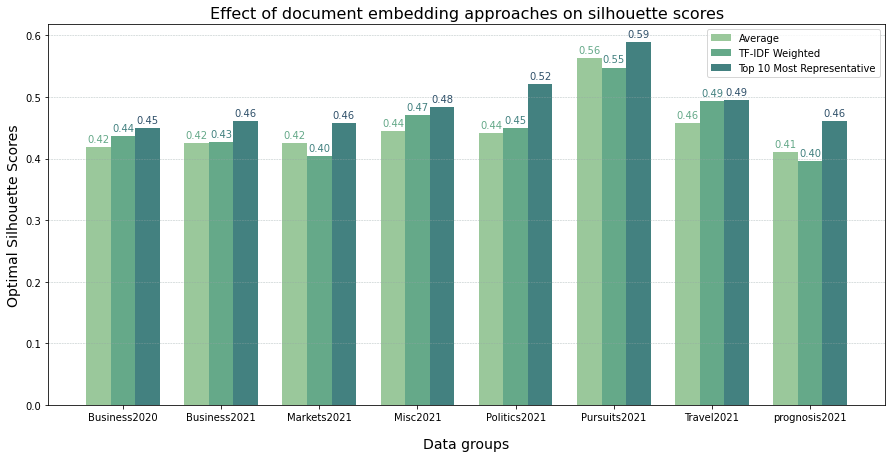
\includegraphics[width=0.9\linewidth]{images/eval/doc_embedding_sil.png}
  \caption{Effect of document vector generation approaches on clustering silhouette scores where Approach 1 = Average, Approach 2 = TF-IDF Weighted, and Approach 3 = Top 10 most Representative }
  \label{fig:doc_embeddings}
  \end{figure}

\Cref{fig:doc_embeddings} shows how the different document (article) embedding approaches effect the `goodness' of the clustering indicated by silhouette scores. The significance of scores on clustering is explained in detail in~\Cref{s:silhouette score} explThe consensus derived is that Approach 3, which describes calculating the article vector by computing the weighted average of the top 10 most relevant words (using the TF-IDF metric), performs better than the other 2 approaches mentioned. Approach 3 results in a 9.36\% improvement in silhouette score compared to Approach 1 (simple averaging of word vectors) and an 8.37\% improvement compared to Approach 2 (weighted (TF-IDF) average of all word vectors). This led to the decision of using Approach 3 as the method for document vector generation.
%  \hl{Figure out how to add the silhouette score stuff before?}

%%%%%%%%%%%%%%%%%%%%%%%%%%%%%%%%%%%%%%%%%%%%%%%%%%%%%%%%%%%%


\subsection{Dimensionality Reduction}

\subsubsection{Normalising Data}

Before performing any dimensionality reduction, first step is to normalise the article vectors in order to eliminate redundancy in data and standardise the features (components of the vector). Clustering article vectors involves minimising a `distance' metric.If different vector components (features) have different scales, derivatives will tend to align along dimensions with higher variance, resulting in poor convergence. For instance, for a given dataset, \hl{if dimension 1 is in the 100s and dimension 2 is in 1s}, then dimension 1 will have a much higher effect on in the overall distance, making the clustering biased towards it. Therefore, normalisation (or feature scaling) is crucial for clustering as it controls variability in data (collection of document vectors), re-scaling the feature components to share a common scale, thereby improving clustering. Additionally, when it comes to performing principal component analysis for the article vectors, the vector components (features) should be independent of their standard deviation or variance to get a good covariance matrix among the features.   

\subsubsection{Principal Component Analysis}

As established previously (See~\Cref{word_embed_approaches}), \texttt{GloVe} embeddings are used for article vector generation. Clustering the document vectors becomes inefficient and meaningless at these high dimensions as the concept of distance becomes less precise when the number of dimensions increases~\cite{pca_clustering}. This is because the volume of space increases exponentially making the available data sparse - `curse of dimensionality'. For any given point in this high n-dimensional space, the difference in `distance' (euclidean) to the closest point $d_{min}$ and the farthest point $d_{max}$ with respect to the $d_{min}$ becomes negligible~\cite{nearest_neighbour}. 

\[ \lim_{n\to\infty} \frac{d_{max} - d_{min}}{d_{min}} \to0\]

The concept of clustering these articles relies on grouping similar articles together based on their features (vector components). However, given the high dimensional data, some of these features are not significantly relevant in determining the clusters. The goal is to find the vector components with the most variance across the documents vectors to represent the features. This is accomplished by performing principal component analysis (PCA) on the normalised high-dimensional input vector space to map it to a lower dimensional space, whilst minimising information loss~\cite{pca_clustering}.

\vspace{-2ex}
\begin{figure}[H]
  \centering
    \begin{minipage}[t]{.49\textwidth}
      \centering
      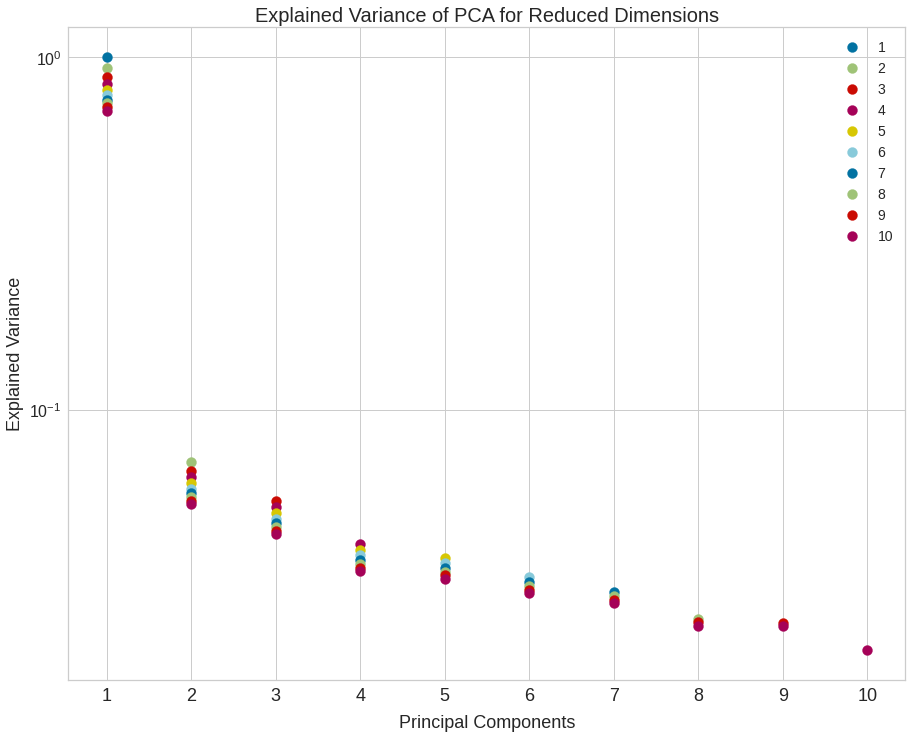
\includegraphics[width=\textwidth]{images/eval/explained_variances.png}
      \caption{Proportion of explained variance across principal components for transformed data to dimensions=1..10}
      \label{fig:explained_variance}
    \end{minipage}
    \begin{minipage}[t]{.49\textwidth}
      \centering
      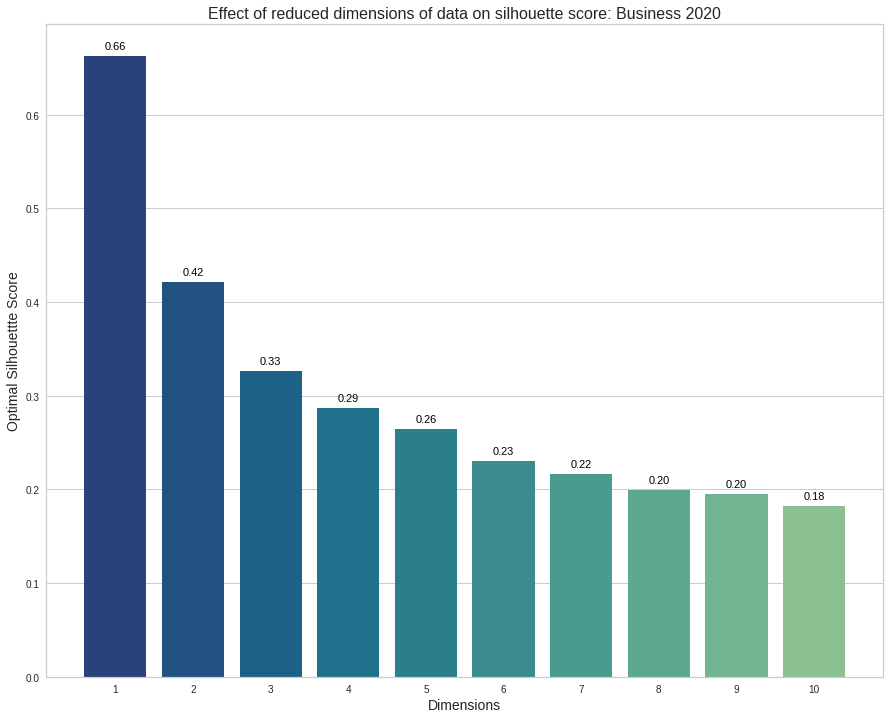
\includegraphics[width=\textwidth]{images/eval/pca_silhouette.png}
      \caption{Optimal silhouette scores for data with dimensions=1..10 transformed using PCA }
      \label{fig:pca_sil}
    \end{minipage}
  \end{figure}


  As seen in~\Cref{fig:explained_variance}, when the article vector space is projected to dimension=1, the variance is explained entirely by the 1$^{st}$ principal component (indicated by the blue dot). As the number of dimensions increase, i.e. the number of principal components increase, the main proportion of the variance (close to 1) can still be explained by the first principal component. Projecting to 10 dimensions, the proportion of explained variances (as a percentage) for each of the 10 principal components is as follows: 
  \begin{table}[H]
      \centering
  \renewcommand{\arraystretch}{1.1}
  \begin{tabularx}{\textwidth}{|X|X X X X X X X X X X|} 
    \hline
    PC & \textbf{1} & \textbf{2}  & \textbf{3}  & \textbf{4}  & \textbf{5} & \textbf{6} & \textbf{7}  & \textbf{8}  & \textbf{9}  & \textbf{10}\\
    \hline
    EV(\%) & 70.6\% & 5.4\% & 4.4\% & 3.5\% & 3.3\% & 3.0\% & 2.8\% & 2.4\% & 2.4\% & 2.1\% \\ 
    \hline
    \end{tabularx}
  \end{table}

  Therefore, even at 10 dimensions, 70.6\% of the variance can be explained by the first principal component (PC) alone and therefore, the article vector space can be transformed using PCA with dimensions=1. \Cref{fig:pca_sil} shows the effect of transforming the article vector space to different dimensions on the silhouette scores, which represent the `goodness of clustering'(See~\Cref{s:silhouette score}). It indicates that transforming the vectors to a single dimension (using PCA) result in the highest silhouette score. Therefore,~\Crefrange{fig:explained_variance}{fig:pca_sil} conclude that the setting the dimension to 1 for PCA transformation results in the most optimal clustering whilst minimising information loss.

\subsection{KMeans Clustering}
Once the normalised data is mapped to the lower subspace, the articles are clustered based on their cosine similarity~\cref{eq:cosine_sim} using `cosine distance' as the distance function~\cref{eq:cosine_distance} and KMeans as the clustering technique. This was done using the \texttt{kmeans} function exposed by the \texttt{sklearn} library but `euclidean distance'~\cref{eq:euc_distance} (instead of `cosine distance') as distance metric. This is feasible given the linear relationship between euclidean distance and  cosine distance~\cite{kmeans} for normalised vectors shown in~\cref{eq:relationship_ce}.

\begin{align}
  \mathit{For \ normalised \ vectors,} \ x, y:  \sum x_i^2 &= 1,  \sum y_i^2 = 1 \label[equationX]{eq:normalised} &\\ 
  \mathit{Cosine \ Similarity,} \ cos(x, y) &= \frac{\sum x_i y_i}{\sqrt{\sum x_i^2 y_i^2}}  \nonumber &\\ 
   &= \sum x_i y_i \label[equationX]{eq:cosine_sim} &\\
   \mathit{Cosine \ Distance} &= 1 - cos(x, y) \label[equationX]{eq:cosine_distance} &\\
   \mathit{Euclidean \ Distance,} \ || x - y ||_2^2  &= \sum (x_i -  y_i)^2  \label[equationX]{eq:euc_distance} &\\
                 &= \sum (x_i^2 + y_i^2 - 2 x_i y_i)  \nonumber &\\
                 &= \sum x_i^2 + \sum y_i^2 - 2\sum x_i y_i   \nonumber &\\
                 &= 1 + 1 - 2 cos(x, y)  \nonumber &\\
                 &= 2 (1 - cos(x, y))  &\\
                 &= 2 (\mathit{Cosine \ Distance}) \label[equationX]{eq:relationship_ce}
\end{align}


% \todonum[inline, color=darkgray]{Add kmeans formula - MDS?}

Furthermore, to avoid falling into the trap of random centroids initialization, a major shortcoming of the KMeans method, the clustering was done with KMeans++. KMeans++ offers a better initialisation approach for centroids, in which the first one is picked at random and the subsequent centroids are chosen with a probability proportional to the squared distance from the closest chosen centroid.


\subsection{Determining the optimal number of clusters} \label{s:optimal_clusters}
Determining the number of clusters (k) in KMeans is a crucial factor to consider. This was done by computing the KMeans clustering algorithm for different values of k varying from 2 (minimum number of clusters) to m (maximum number of clusters), and picking the optimal k based on a comparing statistic. The two comparison statistics considered were: Elbow method with Within Cluster Sum of Square distance (WCSS) and Silhouette score. 

\subsubsection{Method 1: Minimising WCSS using Elbow Method}
The elbow method uses the distance (Euclidean) between the cluster centroid and its members, i.e., intra-cluster variance (also known as, distortion score or WCSS) to determine how many clusters are needed to encapsulate the variance of the data. In particular, it minimises the loss function: WCSS (or distortion score) which is the sum of the squared distance between each point in a cluster from its corresponding centroid~\cite{elbowvssil} as shown in~\ref{eq:wcss}.
% \newenvironment{where}{\noindent{}where\begin{itemize}}{\end{itemize}}

\vspace{-2ex}
\begin{gather}
  \mathit{WCSS} =  \sum^{C_n}_{C_k} (\sum^{d_m}_{d_i \in C_i} || d_i - C_k ||_2^2) \label[equationX]{eq:wcss} \\
  \text{where~$C$ is the cluster centroid and~$d$ is the data point in each cluster.} \nonumber
\end{gather}
% \begin{where}
%   \item 
% \end{where}

As seen in~\Cref{fig:elbow}, the elbow (bend) in the plot determines the optimal number of clusters, i.e., the k value = 4. The main drawback of using the lowest distortion score to determine the optimal number of clusters is that as long as the number of clusters (k) increases, the distortion score (WCSS) will decrease because the points will be closer to their centroids. Hence, the elbow (bend) is used to determine the minimum number of clusters with a reasonably low distortion score as seen in~\Cref{fig:elbow}, which gives the optimal number of clusters, k=4.

\begin{figure}[H]
\centering
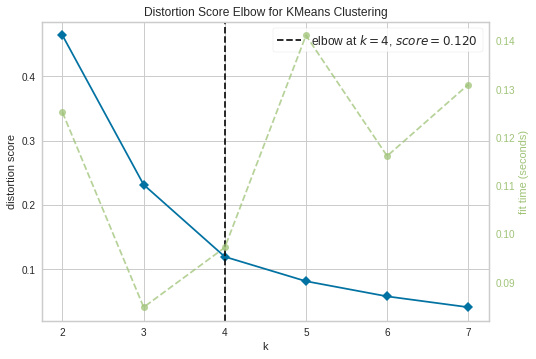
\includegraphics[scale=0.4]{images/elbow.png}
\caption{Elbow Method Plot for KMeans clustering with k=2..7 for input group: `Business 2020' }
\label{fig:elbow}
\end{figure}

\vspace*{-1ex}
\subsubsection{Method 2: Silhouette score} \label{s:silhouette score}

The second approach involved using the silhouette score. Unlike the elbow method, the silhouette score accounts for both how `close' a point is within its cluster (cohesion)~\cite{elbowvssil} as well as how close it is to other clusters (separation)~\cite{silhouette}.
\begin{gather}
  \mathit{Silhouette \ Score} = \mathit{mean}_i (\frac{S_i - C_i}{\max(S_i, C_i)}) \label[equationX]{eq:ss} \\
  \text{where~$cohesion, C_i$} = \text{average distance between data point~$i$ and all points within its cluster} \nonumber \\
  \text{$separation, S_i$} = \text{average distance between data point~$i$ and all points not in its cluster}\nonumber
\end{gather}

The silhouette score for a clustering as shown in~\ref{eq:ss} is the mean of the silhouette score for all points $i$ in the data. It ranges from -1 to 1. A score near 1 implies that clusters are well separated and distinct, while a score close to 0 implies that there is extensive overlapping between the clusters and that the clusters cannot be differentiated. Finally, a score close to -1 implies that clusters are incorrectly assigned.

\begin{figure}[H]
\centering
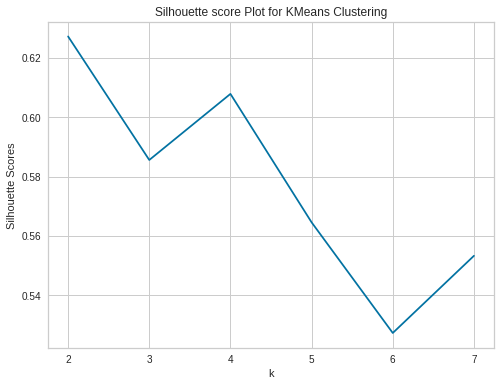
\includegraphics[width=0.4\linewidth]{images/sil_kmeans_.png}
\caption{Silhouette Plot for KMeans clustering with k=2..7 for input group: `Business 2020'}
\label{fig:sil_kmeans}
\end{figure}
\vspace{-2ex}

\begin{figure}[H]
\begin{minipage}{0.49\linewidth}
\centering
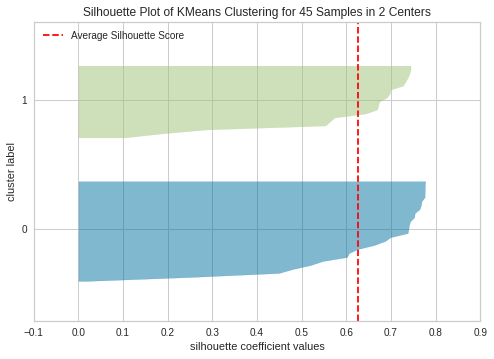
\includegraphics[width=\linewidth]{images/cluster 2.png}
\caption{`Business 2020' Silhouette Diagram: score = 0.627 for k=2}
\label{fig:cluster2}
\end{minipage}
\hfill
\begin{minipage}{0.49\linewidth}
\centering
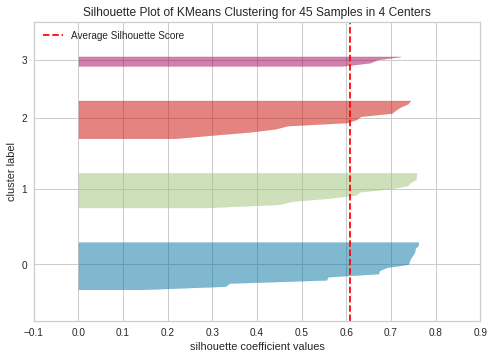
\includegraphics[width=\linewidth]{images/cluster 4.png}
\caption{`Business 2020' Silhouette Diagram: score = 0.607 for k=4}
\label{fig:cluster4}
\end{minipage}
\end{figure}

\vspace*{-1.5ex}
From~\Cref{fig:sil_kmeans}, it is apparent that although selecting k=4 (as found by Elbow Method in~\Cref{fig:elbow}) results in a good clustering, a better clustering can be achieved by selecting k=2, as it gives a higher silhouette score, suggesting less overlap. \Crefrange{fig:cluster2}{fig:cluster4} show the silhouette diagram for number of clusters, k=2 and k=4 respectively. The cluster thickness denotes the size of the cluster, and the width represents the sorted silhouette coefficients of instances in the cluster. Observing~\Cref{fig:cluster2} (k=2) reveals that both clusters are roughly equal in size, whereas~\Cref{fig:cluster4} (k=4), illustrates a higher disparity in size as Cluster 3 is less than half the size of others. This is indicative of some clusters being split, thereby resulting in a suboptimal silhouette score. 

Out of the two approaches, the decision was made to go with silhouette score as the clustering comparison statistic as it factors both how compact a cluster is and how distinct it is. This is a vital consideration given that the aim of the Topic Extraction Engine is to distinctly cluster the news articles with minimal overlap, in order to minimise common topics within clusters post topic modelling (performed on each cluster). 

\subsection*{Find n most representative docs} \label{sec:Find_n_docs}

Once the articles are clustered, the goal is to obtain the cluster-to-article mapping. However, given the high volume of data, considering every single article in the cluster is not necessary, particularly those that are far from their respective cluster centroids. Therefore, the articles are sorted in increasing order of (euclidean) distance from the centroid and the `top n' articles are selected for each cluster. Furthermore, since the next step in the Topic Extraction Engine entails modelling topics on these semantic clusters, it is futile to consider the sparse clusters that have very few (less than $n_{min}$) members as they will not spawn any good topics and are therefore omitted. The $n_{max}$ and $n_{max}$ values are computed based on the mean and standard deviation of the sizes of semantic clusters, $|C|$, as shown in~\crefrange{eq:nmin}{eq:nmax}.
\vspace{-1.5px}
\begin{align}
  n_{min} &= \lfloor mean(|C_1|, |C_2|, ..., |C_n|) - std(|C_1|, |C_2|, ..., |C_n|) \rfloor \label[equationX]{eq:nmin} &\\
  n_{max} &= \lceil mean(|C_1|, |C_2|, ..., |C_n|) + std(|C_1|, |C_2|, ..., |C_n|) \rceil \label[equationX]{eq:nmax}
\end{align}

\section{Topic Modelling}

Post semantic clustering, the aim is to extract topics associated with each cluster. This was done through topic modelling, which follows an unsupervised approach of extracting the top topics from a corpus. In particular, the model used was the Latent Dirichlet allocation (LDA) from the Gensim library. 

As explained in~\Cref{Topic Modelling appoaches}, each document (`article intro') is made up of several words (\texttt{filtered\_tokens}) and each topic has several (key)words associated with it. Given that LDA is a probabilistic model, it tries to estimate the topic distribution for each article as well as the word distribution for each topic. The motivation for using LDA is to get the topic-document probability distribution which can then be used to get the topics associated with an article. For the scope of this problem, each article was associated with one dominant topic. 

It is important to note that topic modelling LDA does not rely on semantic information, this is why the decision was made to obtain semantic clusters first and then model topics on them.
\vspace{-1ex}
\subsection{Corpus Decisions}

From the data processing steps detailed in~\Cref{s:procesing_topic_engine}, the `article intros' have already been cleaned, lemmatised, filtered and tokenised to get their corresponding \texttt{filtered\_tokens}, which are void of any stopwords and named entities and only contain nouns. For the input corpus passed to the LDA, there were certain key decisions made, which were influenced by previous studies and quantitive evaluation (discussed in~\Cref{s:evaluation_topic_extraction}). Using the \texttt{filtered\_tokens} satisfied most of these requirements which are explained below: 

\begin{enumerate}
  \item \textbf{Noun-only corpus}: Based on previous studies~\cite{nouns_only_lda}~\cite{efficient_noun_only_approach}, and the results from~\Cref{s:pos_topic} which saw improved coherence values of topics averaged across clusters and fewer numbers of `unpopular' topics (i.e. those with few associated articles), the decision was made to limit input corpus to nouns (satisfied by \texttt{filtered\_tokens}). This aligned with the intuition that nouns are better indicators of a topic as they provide more semantic context. Opening the corpus to other POS categories, for instance, ADJ, VERB (See Appendix~\Cref{appendix:pos}), resulted in sub-optimal topics since the LDA model will give ``fast" and ``pandemic" equal importance.
  
  \item \textbf{No Named Entities}: Similar to semantic clustering, the decision was made to omit all named entities from the LDA corpus. This was also satisfied by the \texttt{filtered\_tokens} where the entities found using the Fine-Grained NER model were removed. As seen in ~\Cref{fig:pos_topic}, omitting named entities improved the coherence score of the topics. The aim for this was to prevent the LDA model from fitting topics to named entities instead of common nouns (which indicate key themes in corpus). 

  \item \textbf{Using Bigrams}: Inspired by \cite[`Beyond bag of words']{bigrams_lda}, a decision made was to augment the corpus using n-grams, in particular, bigrams, rather than solely using unigrams. This allowed the model to consider a combination of two commonly occurring words across documents, e.g., ``coronavirus\_pandemic'', ''aviation\_industry'' etc. This was particularly relevant given that news articles often contain common `noun chunks' which can be used to infer topics. The bigrams are derived using Gensim's \texttt{Phraser} which uses colocation detection, and are appended to \texttt{‘filtered\_tokens’.}
  
  \item \textbf{TF-IDF}: In LDA, the documents need to be transformed into numeric feature vectors which form the input corpus. Since it does not rely on the article's semantic information and builds topic estimators based on words, article and topics, it uses frequency vectors obtained by Bag-of-Words or Term Frequency-Inverse Document Frequency (TF-IDF). The latter was chosen over the more common Bag-of-Words~\cite{topic_models}, in an attempt to minimise overlap of topics as each article will be associated with one dominant topic.
\end{enumerate}


\subsection{Determining number of latent topics}

A key contributor in determining the quality of the topics extracted is tuning the \texttt{num\_topics} parameter \texttt which represents number of topics outputted by the LDA. A low value will result in too few or overly generalised topics whereas a high value results in uninterpretable topics that ideally should have been merged~\cite{topic_score}. Previous studies~\cite{cv_abstract}~\cite{cv_space} show that one of the best methods to determine the number of latent topics is to measure CV coherence, which has a high correlation with human judgments of topic interpretability. This metric computes the normalised pointwise mutual information (NPMI) and cosine similarity of content vectors of words, derived based on their co-occurrences~\cite{cv_space}.

This was achieved by using \texttt{CoherenceModel} with the `c\_v' setting from the Gensim library. The optimal number of topics (i.e., value resulting in the highest coherence score) is computed for each cluster by running the LDA model with different values of k varying from min\_topics (defaulted to 2) to max\_topics (which is dependent on the size of the semantic cluster). The LDA model with the highest resulting coherence is chosen. The motivation for bounding the max\_topics was to ensure topics would have at least the minimum number of `article intros' (=2). Additionally, pruning the number of LDA runs reduces unnecessary computation, improving performance.

\subsubsection*{Dominant Topic-Article Mapping} \label{sec:topic_article_mapping}
Once the optimal value of \texttt{num\_topics} is determined, the corresponding LDA model is applied to the TF-IDF corpus to get the resulting article-topic distribution. This returns the most probabilistic topics for each article intro. This is of the form \texttt{articleId: (topicId, probability)}, where \texttt{probability} refers to the likelihood that the article belongs to the topic corresponding to the \texttt{topicId}. Of these, the most dominant topic (the highest likelihood of the article belonging to the topic) is selected, resulting in an 1-1 topic-article mapping. 

\vspace{-1ex}
\subsection{Topic Name Inference}

An augmented feature of the Topic Modelling Engine was to infer the topic names from the topic keywords. \Cref{alg:topic_name} details this process. This involves splitting any bigram keywords to obtain a set of keyword tokens which are validated to ensure they are nouns, not a stopword and have an associated \texttt{Glove} embedding. Using the \texttt{GloVe\_model.most\_similar()} method from Gensim, which computes the cosine similarity between an average of projection of resulting keyword vectors (\texttt{validKws}), the candidate topic names are obtained. These are again enforced to be nouns and checked against the augmented stopwords (See~\Cref{data_cleaning}). The top 3 most similar topic name tokens that meet the validity checks are selected as the `topic name' for the given topic. If there are no valid \texttt{topic\_name\_candidates}, the first valid keyword is used as the topic name as the keywords from the LDA are outputted in descending order of importance.

\begin{algorithm}[H]
  \caption{Infer Topic Name}
  \label{alg:topic_name}
  \begin{algorithmic}   
    \Function{GetValidKeywords}{$\mathit{topicKeywords, stopwords, allowed\_pos=}$[`$\mathit{NOUN}$']}
    \State $\mathit{validKws} \gets \emptyset$
    \ForAll{$\mathit{topicKw} \in \mathit{topicKeywords}$} 
    \State $kw \gets \mathit{topicKw.lemma}$
    \If {$kw \in stopwords$ \AND $kw \notin GloVe.vocab$ \AND $kw.pos \notin allowed\_pos$}
    \State $continue$
    \EndIf
    \State $validKws.append(kw)$
    \EndFor
    \State \Return $validKws$
  \EndFunction

\vspace{1em}
  \Function{GetTopicName}{$topicKeywords$, $stopwords$}
    \State $kws \gets$ \Call{GetKeywordTokens}{$topicKeywords$}
    \Comment{$splits \ bigrams$}
    \State $validKws \gets$ \Call{GetValidKeywords}{$kws, stopwords}[:5]$
    \State $\mathit{topicNameCandidates} := \mathit{GloVe.most\_similar(validKws, topn=5)}$
    \State $\mathit{validTopicNames} \gets$ \Call{GetValidKeywords}{$topicNameCandidates, stopwords$}
    \If {$len(validTopicNames) == 0$}
    \State \Return $validKws[0]$
    \Else
    \State \Return $validTopicNames[0:2]$
    \EndIf
  \EndFunction
\end{algorithmic}
\end{algorithm}

\vspace{-2em}
\subsection{Topic Sentiment}

The last component of the Topic Modelling Engine involves sentiment analysis. In order to compute the topic sentiment, the sentiment of each article associated with the topic is computed. In order to obtain the article sentiment, the RoBERTa model trained on Stanford Sentiment Treebank (See~\Cref{s:models}) is used on the (coreference resolved) article `title' without any data cleaning (See~\Cref{data_cleaning}). Data cleaning is omitted because removing stopwords for sentiment analysis is often not a good idea as it can it change the meaning of the text, especially by eliminating negations such as `not', `n't' etc. hl{By not restricting the input to nouns, the model is able to account for the adjectives and adverbs that contribute to the strength of the sentiment associated with a particular entity.} The article `title' is used instead of the entire article as the title provides the main topic sentence for the article, serving a as good descriptor of the tone of article. News articles mention several target entities (some more relevant than others)and the sentiment around each of these will equally influence the overall article sentiment. This diverts focus from the main point of the article (summarised nicely by the title), resulting in a sentiment that does not coincide with the key tone of the article as it is influenced by too much noise.

Given that the model is a binary classifier, it produces a binary label, where 0 represents 'negative' sentiment and 1 represents 'positive' sentiment. The sentiments of the articles linked with a topic are then averaged, and the topic is assigned one of three sentiments based on the range of the resulting value: 'Positive,' 'Negative,' or 'Neutral' as shown in~\Cref{alg:topic_sent}.

\begin{algorithm}[H]
  \caption{Computing Topic Sentiment}
  \label{alg:topic_sent}
  \begin{algorithmic}   
  \Function{GetTopicSentiment}{$topicArticles$}
    \State $sentiments \gets  \emptyset$
    \ForAll {$article \in topicArticles$}
    \State $\mathit{sentiments.append(roBERTa\_model.predict(article.title))}$ \Comment{$0: N, 1:P$}
    \EndFor
    \State $avgSent = average(sentiments)$
    \If {$avgSent >= 0.4 \AND avgSent <= 0.6$}
    \State \Return `$Neutral$'
    \ElsIf {$avgSent > 0.6$}  \Return `$Positive$'
    \Else  \State \Return `$Negative$'\EndIf
  \EndFunction
\end{algorithmic}
\end{algorithm}
\vspace*{-3ex}

\section{Results and Discussion}

For topic extraction, usually one of either cluster analysis or topic modelling is performed on the input data (in this case, news articles), however, by combining these methods we are able to provide a high-level semantic grouping through clustering as well as a finer-grained grouping through topic models (using LDA), thereby improving the coherence of these the extracted latent topics. Using POS filtering, stopword removal, lemmatisation and TF-IDF to pre-process the LDA corpus allows for distinct topics with minimal overlap in the semantic clusters (indicated through relatively high coherence scores in~\Cref{s:evaluation_topic_extraction}). The confidence in this approach is obtained through qualitative analysis of the results from the Topic Extraction Engine which are displayed by the visualisation tool as shown in~\Crefrange{fig:topics_travel2021}{fig:topics2_travel2021}.
\vspace{-1ex}
\begin{figure}[H]
  \centering
  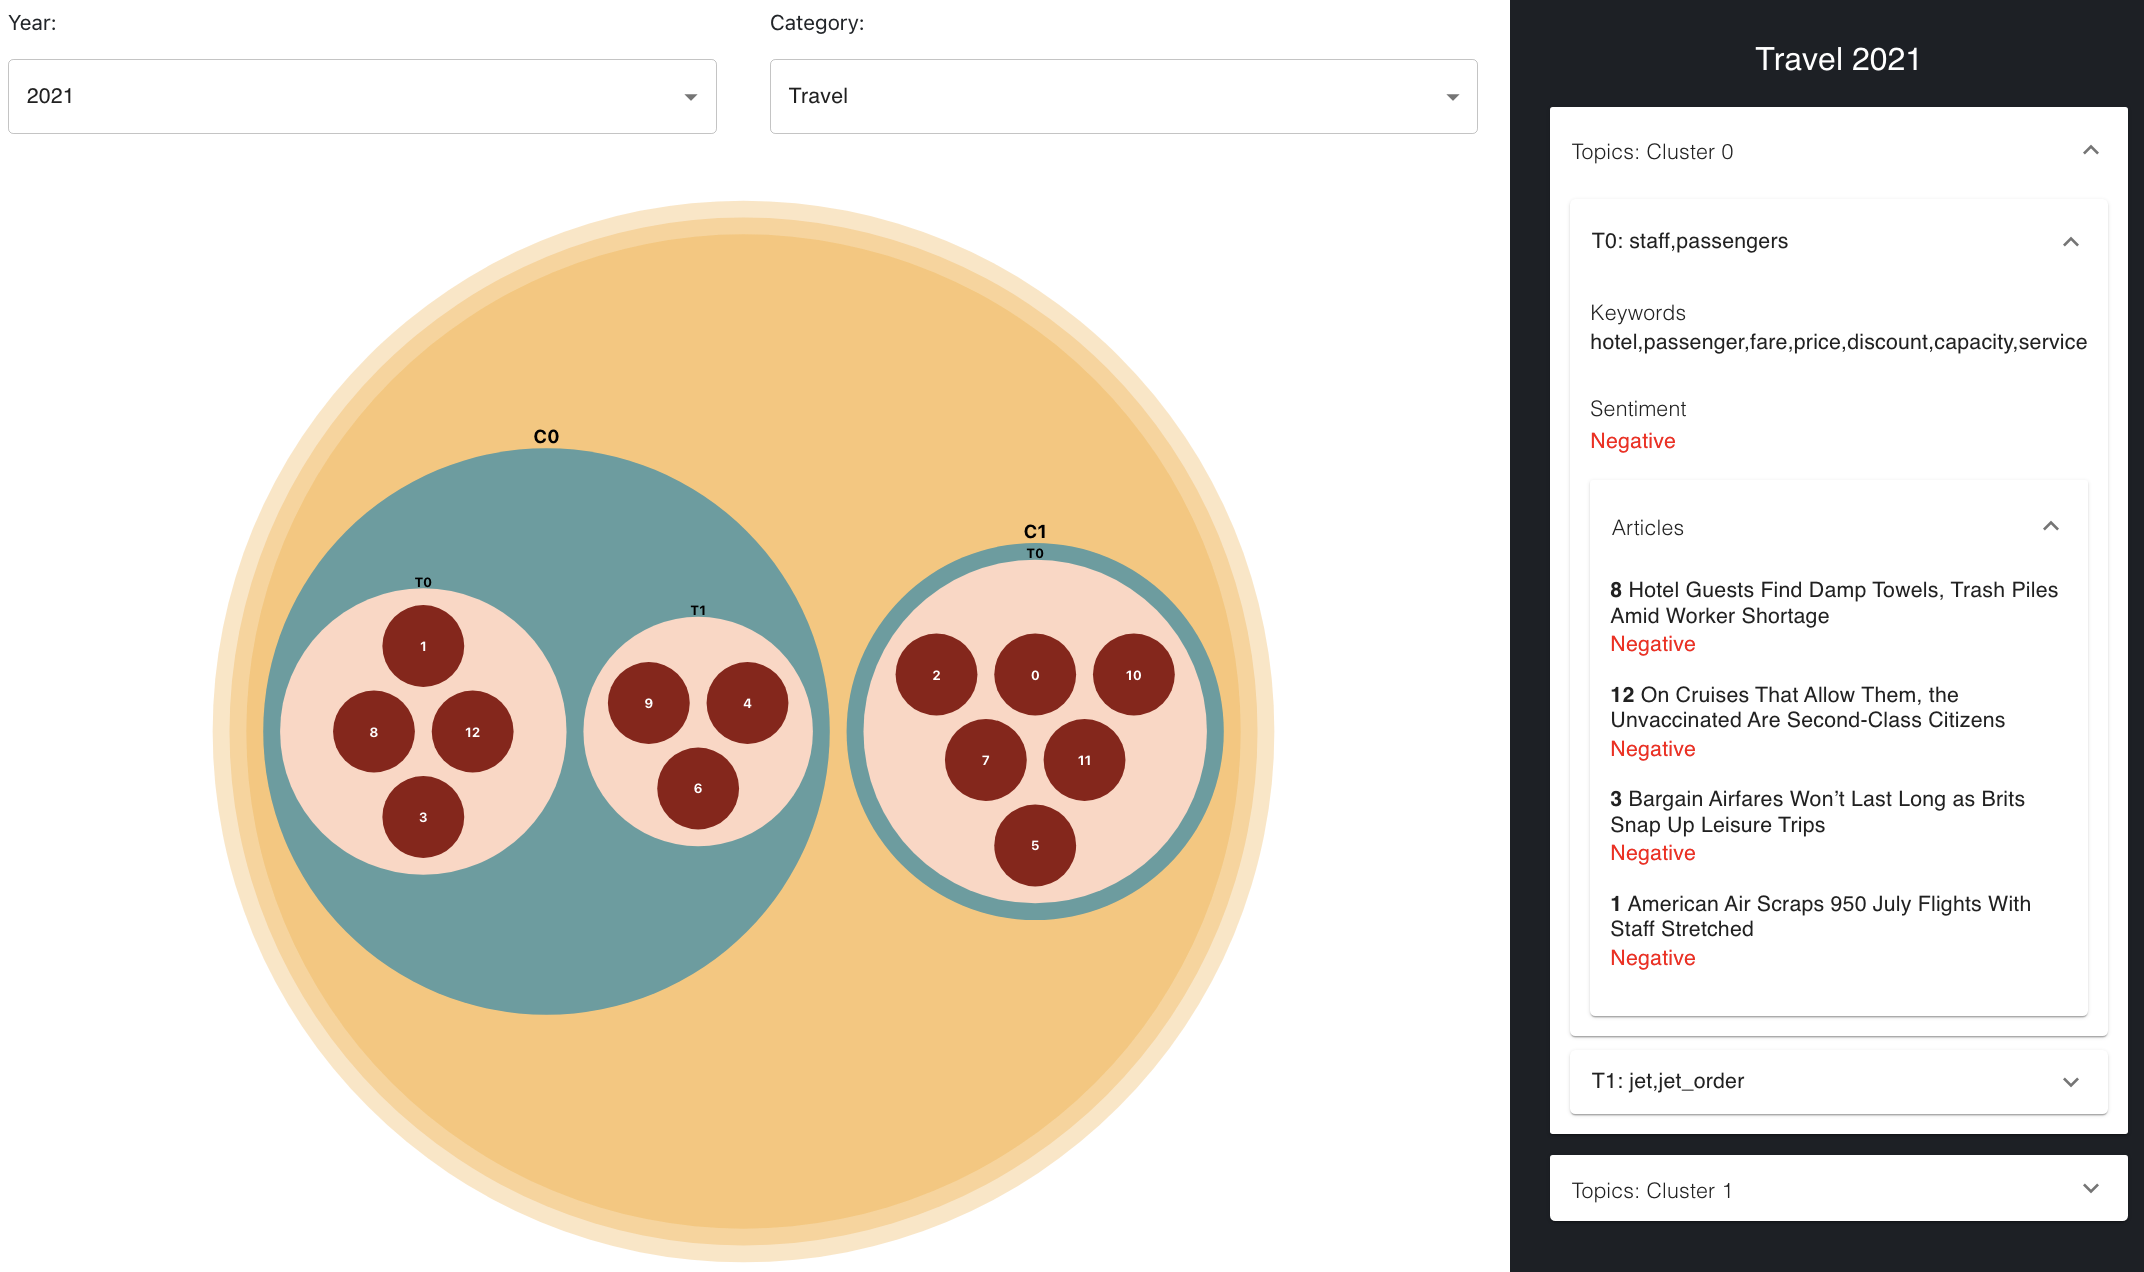
\includegraphics[width=0.93\linewidth]{images/travel2021_topics_cropped.png}
  \caption{Cluster-Topic diagram for Cluster 0 (C0) in `Travel 2021', with expanded view displaying topic information for topic T0}
  \label{fig:topics_travel2021}
\end{figure}

The aim of the Topic Extraction Engine is to derive semantic clusters from the article corpus for each Year-Category group, apply topic modelling on each of these clusters to obtain meaningful, isolated latent topics (represented by the `topic name' and `keywords') and provide topic information such as topic sentiment and associated articles. Additionally, we want to maintain that the distinction among the clusters is signifiant and intuitive by way of the topics within them.  

\Cref{fig:topics_travel2021} displays the `cluster-topic' graph for `Travel2021' which has 2 semantic clusters `C0' and `C1', with 2 and 1 topics respectively. In particular, this figure displays the expanded `accordian' for the first topic `T0' for Cluster 0 (`C0'). This particular input group contained limited data and is used as an example for ease of understanding. We can see that topic (T0) in Cluster 0 (C0) has the inferred topic name of `staff, passengers' with the topic keywords: `hotel', `passenger', `fare', `price', `discount', `capacity' and `service'. The articles within this topic (numbered 1,3,8,12) all talk about passengers (`Hotel Guests' in article 8, `cruise' passengers in article 12, `British' passengers in article 3) and staff (`worker shortage' in article 8 and `staff stretched' in article 1). The keywords are also indicative of the general theme of the articles in the topic. All the articles in this topic are have `negative' sentiment as they generally focus on airlines struggling with poor service due to worker shortage, resulting in an average `negative' sentiment for the topic.

\begin{figure}[H]
  \centering
  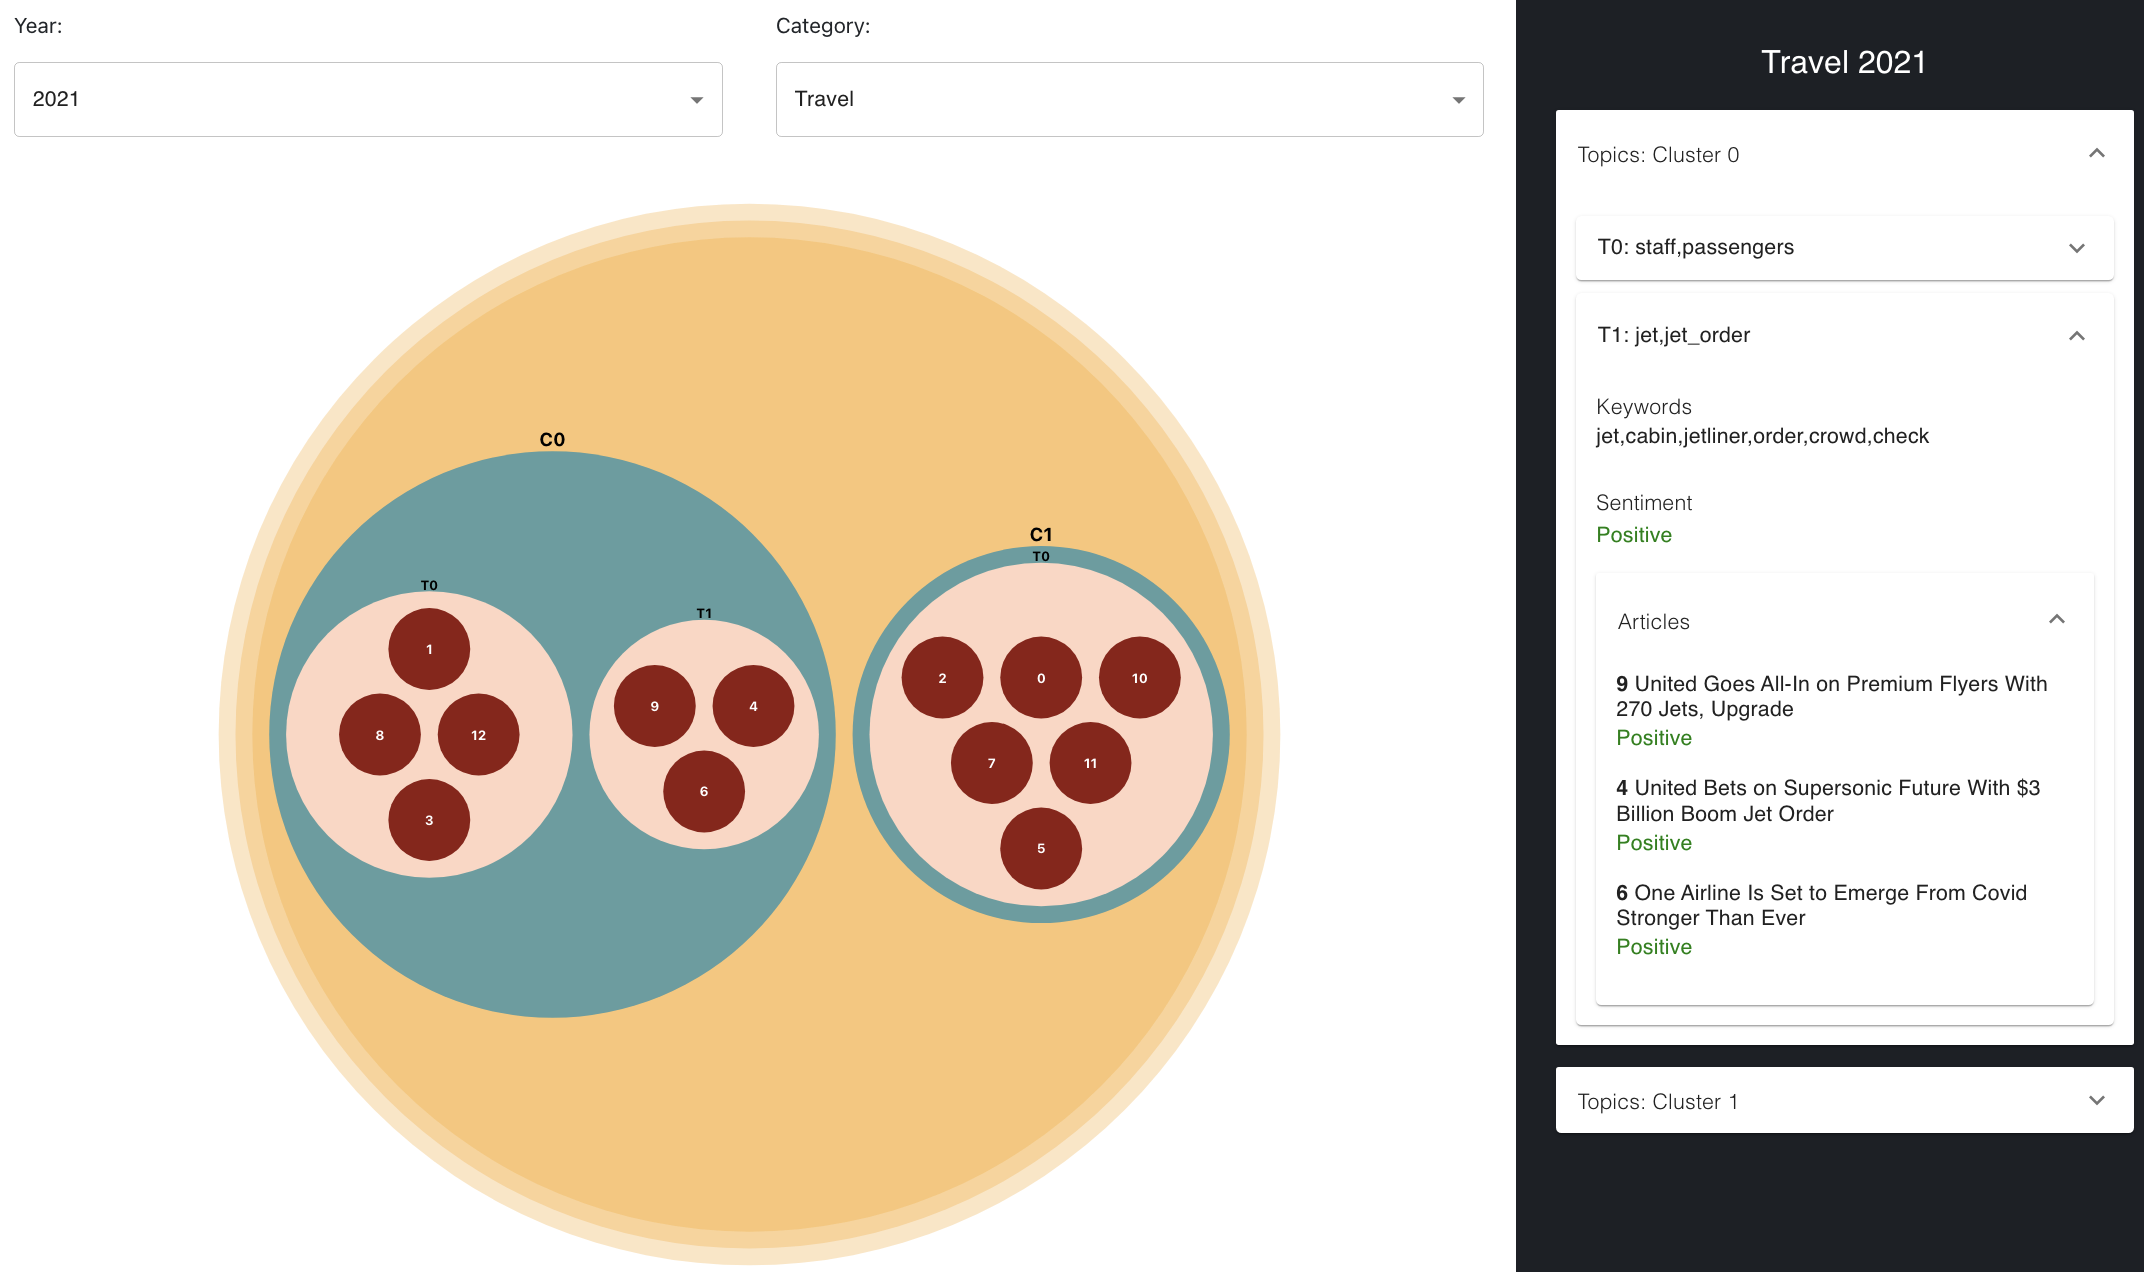
\includegraphics[width=0.99\linewidth]{images/travel2021_topics_1b.png}
  \caption{Cluster-Topic diagram for Cluster 0 (C0) in `Travel 2021', with expanded view displaying topic information for topic T1}
  \label{fig:topics1b_travel2021}
\end{figure}

Similarly, \Cref{fig:topics1b_travel2021}, shows the expanded accordion for the other topic (T1) in the same semantic cluster (C0) with the inferred topic name of `jet, jet\_order' and topic keywords: `jet', `cabin', `order', `jetliner', `crowd' and `check'. This topic differs from the previous topic as this focuses the positive developments made by airlines by investing into new planes and jets. All articles in this topic (numbered 9,4,6) have a `positive' sentiment resulting in overall average `positive' sentiment for this topic.

Therefore, based on the information presented by \Crefrange{fig:topics_travel2021}{fig:topics1b_travel2021} about topics T0 and T1 respectively, for the semantic cluster C0, we can infer that the high-level semantic grouping in C0 focuses on `airlines' and `aircraft' with T0 focusing on the airlines struggling with staff and passenger service and T1 on investment in aircraft through new jet orders. This gives confidence in the Topic Extraction Engine's ability to extract meaningful distinct topics from the article corpus for a given semantic cluster. 


% topic keywords as `country', `tax, `arrival, `state', `reopening' and `tourist'.
\begin{figure}[H]
  \centering
  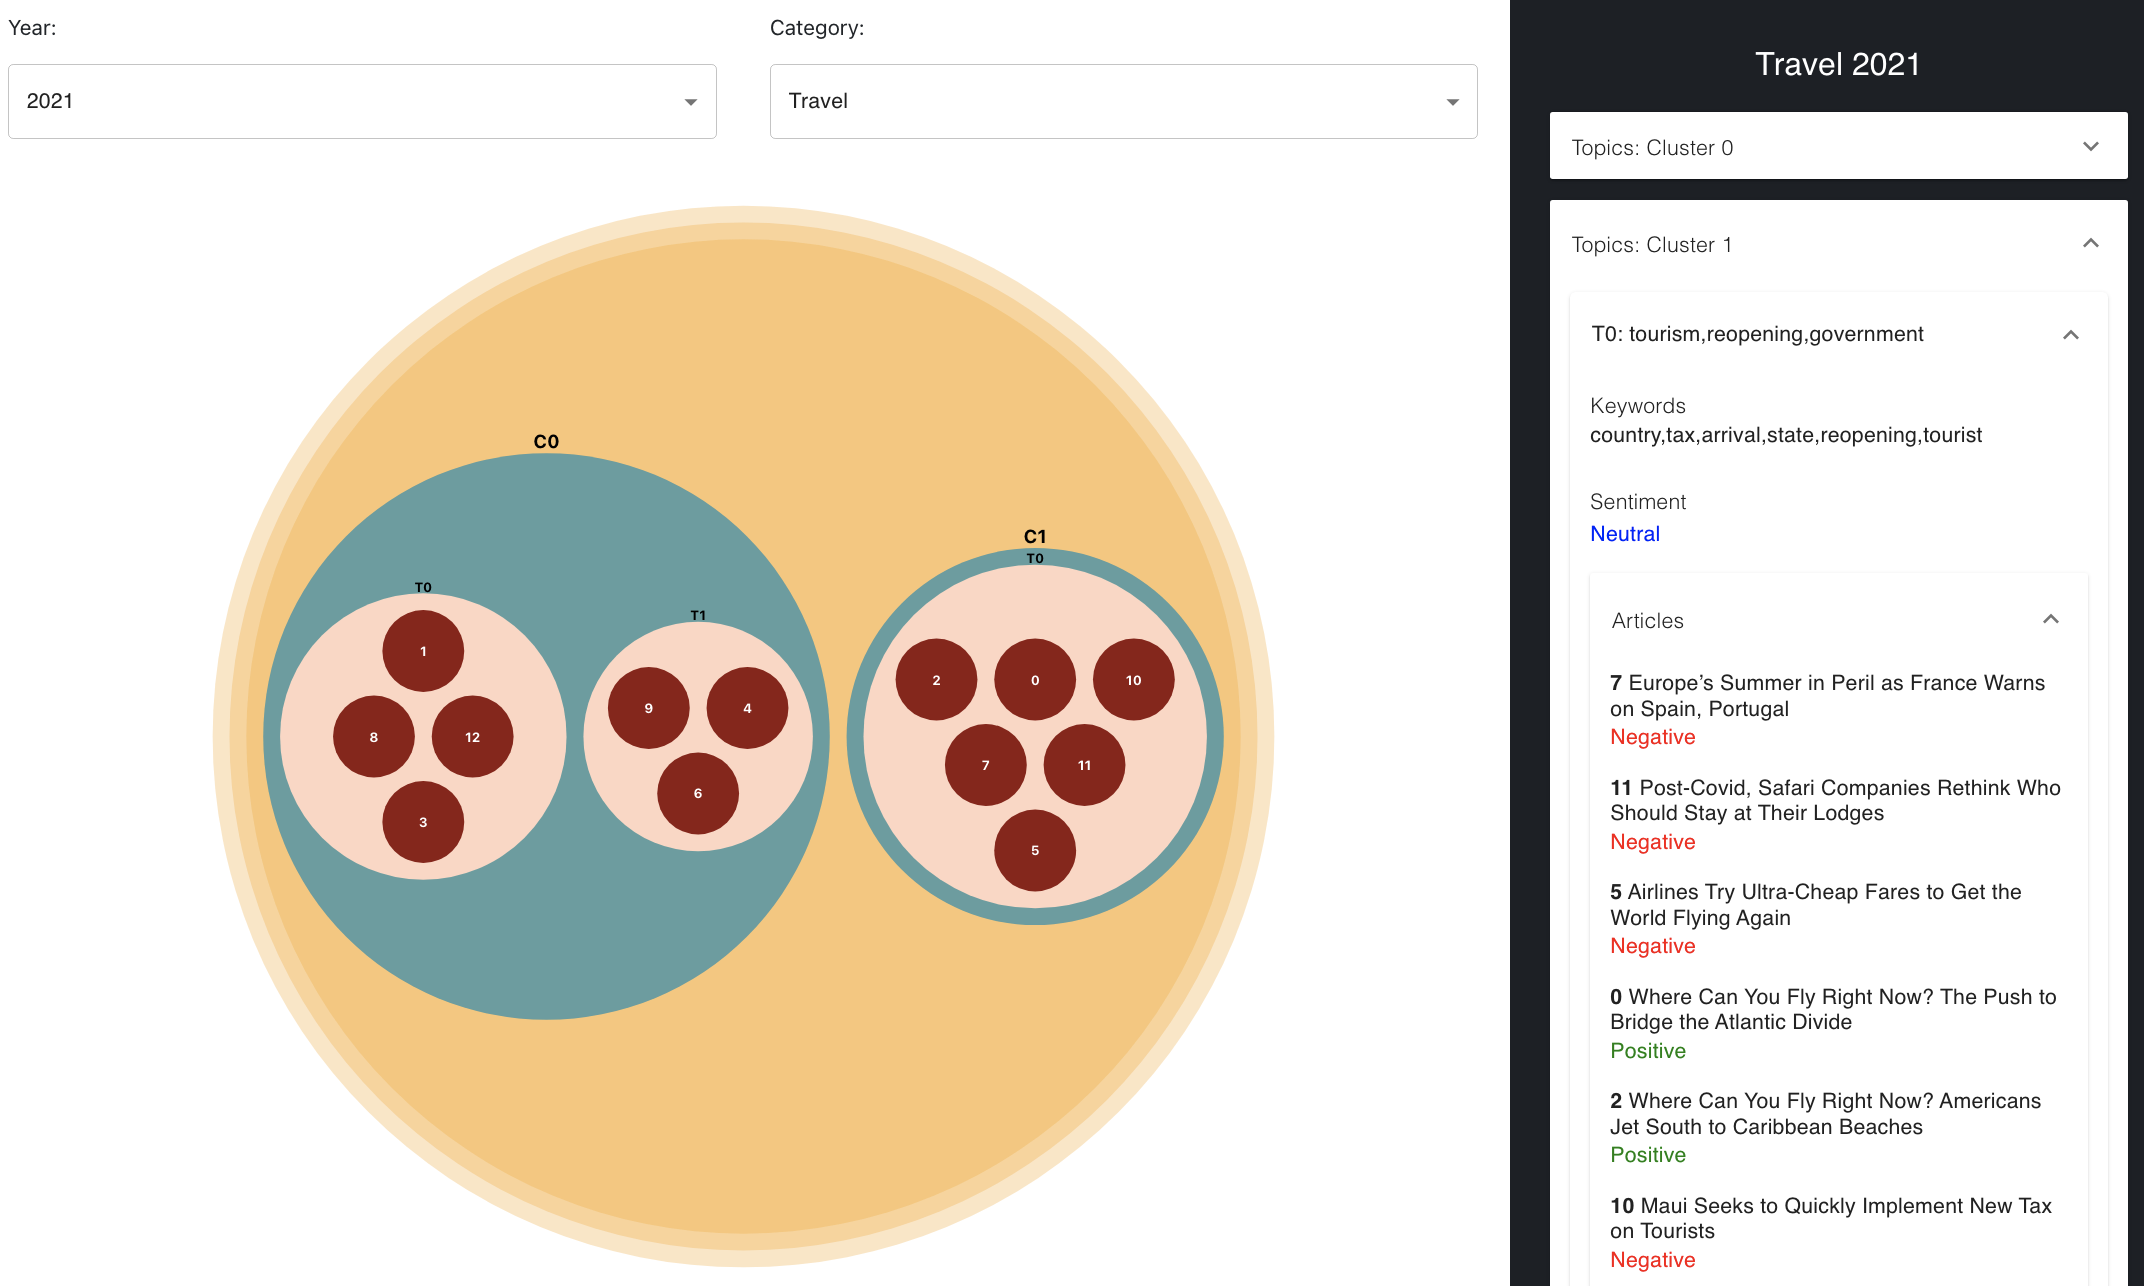
\includegraphics[width=0.99\linewidth]{images/travel2021_topics_2.png}
  \caption{Cluster-Topic diagram for Cluster 1 (C1) in `Travel 2021', with expanded view displaying topic information for the only topic T0}
  \label{fig:topics2_travel2021}
\end{figure}

\Cref{fig:topics2_travel2021} displays the information about a different semantic cluster (C1) which has only one topic (T0) with the inferred topic name `tourism, reopening, government' and keywords: `country', `tax', `arrival', `state', `reopening' and `tourist'. Unlike Cluster 0 (C0), this cluster (and topic) focuses on tourism. The articles associated with topic TO indicate a divided outlook towards airline tourism as some articles talk show reluctance in resuming travel as they talk about implementing new tourist taxes (e.g., article 10) and screening guests post-Covid (e.g., article 11) while other articles imply an eager approach towards promoting tourism as they mention airlines adopting cheaper fares and pushing travel (articles 0,2 and 5). This divided view associated with post-Covid travel is reflected in the sentiments of these articles, thereby resulting in a `Neutral' average sentiment for topic T0 in Cluster 1.

\vspace{2ex}

Therefore, based on results seen in \Crefrange{fig:topics_travel2021}{fig:topics2_travel2021}, we also get confidence in the Topic Extraction Engine's semantic clustering, as we can see the distinction in the different clusters extracted: C0 which focuses on airlines, jet orders and C1, which focuses on resuming tourism.
Furthermore, the qualitative differences between the topics within clusters are is also apparent, which successfully provide insight into the relevant articles contributing to these topics, as well as the associated sentiment regarding that topic.

\subsection{Limitations} \label{limitation_topics}

One of the limitations of the Topic Extraction Engine is the inherent limitation of topic models. There a certain ambiguity associated with the term `topic', while they provide a general grouping of themes in the text, they can not be interpreted as highly nuanced article classification. For topics with several associated articles, it can be sometimes be difficult to interpret the topic, particularly the `topic name'. This is because if the keywords present in the topic have low semantic similarity in terms of their \texttt{GloVe vector embeddings}, the current Topic Name Inference approach is not able to extract a 'meaningful' topic name.

\hl{As mentioned earlier, for the scope of this project, the decision was made that each article is associated with one dominant topic. This can result in the engine omitting certain topics, labelling them insignificant as they do not have sufficient articles associated with them. That may not be true as it may be the case there are sufficient articles that have these as underlying topics, just not the dominant topic.}

Additionally, as expected, the performance of the Topic Extraction is limited by performance of the state-of-the-art models such as SpanBert for coreference resolution, RoBERTa for sentiment analysis and Fine-grained NER for named entity extraction.  